\section{Problem Formulation}
\label{sec:formulation}

\paragraph{Skills, executions and token positions.}
We supply a skill's instructions directly and hold skill selection fixed.
For the same question, the \emph{donor} execution uses the correct skill
and the \emph{receiver} execution uses length-matched text from a fixed
unrelated skill (Appendix~\ref{app:detail}). The skill's token positions, denoted $\mathcal I$, form the
\emph{source span}. For example, a calculator's formula and input
conventions belong to this span. The question does not.
\emph{Readers}, denoted $\mathcal J$, are positions after the source span, including subsequent
prompt tokens and generated answer tokens. Thus receiver names an
execution, whereas reader names a token position that can attend to the
skill. Causal attention prevents a position from reading future tokens,
so tokens before the source cannot read it.

Layers are indexed from zero. The model processes prompt tokens during
\emph{prefill} and generates answer tokens during \emph{decoding}.
We use greedy decoding, which selects the highest-probability next token.
Our main comparison asks what transferring source states restores in the
receiver and what blocking source attention removes from the donor.

% Queue the design graphic within the methods, ahead of the next page top.
\begin{figure*}[t]
\centering
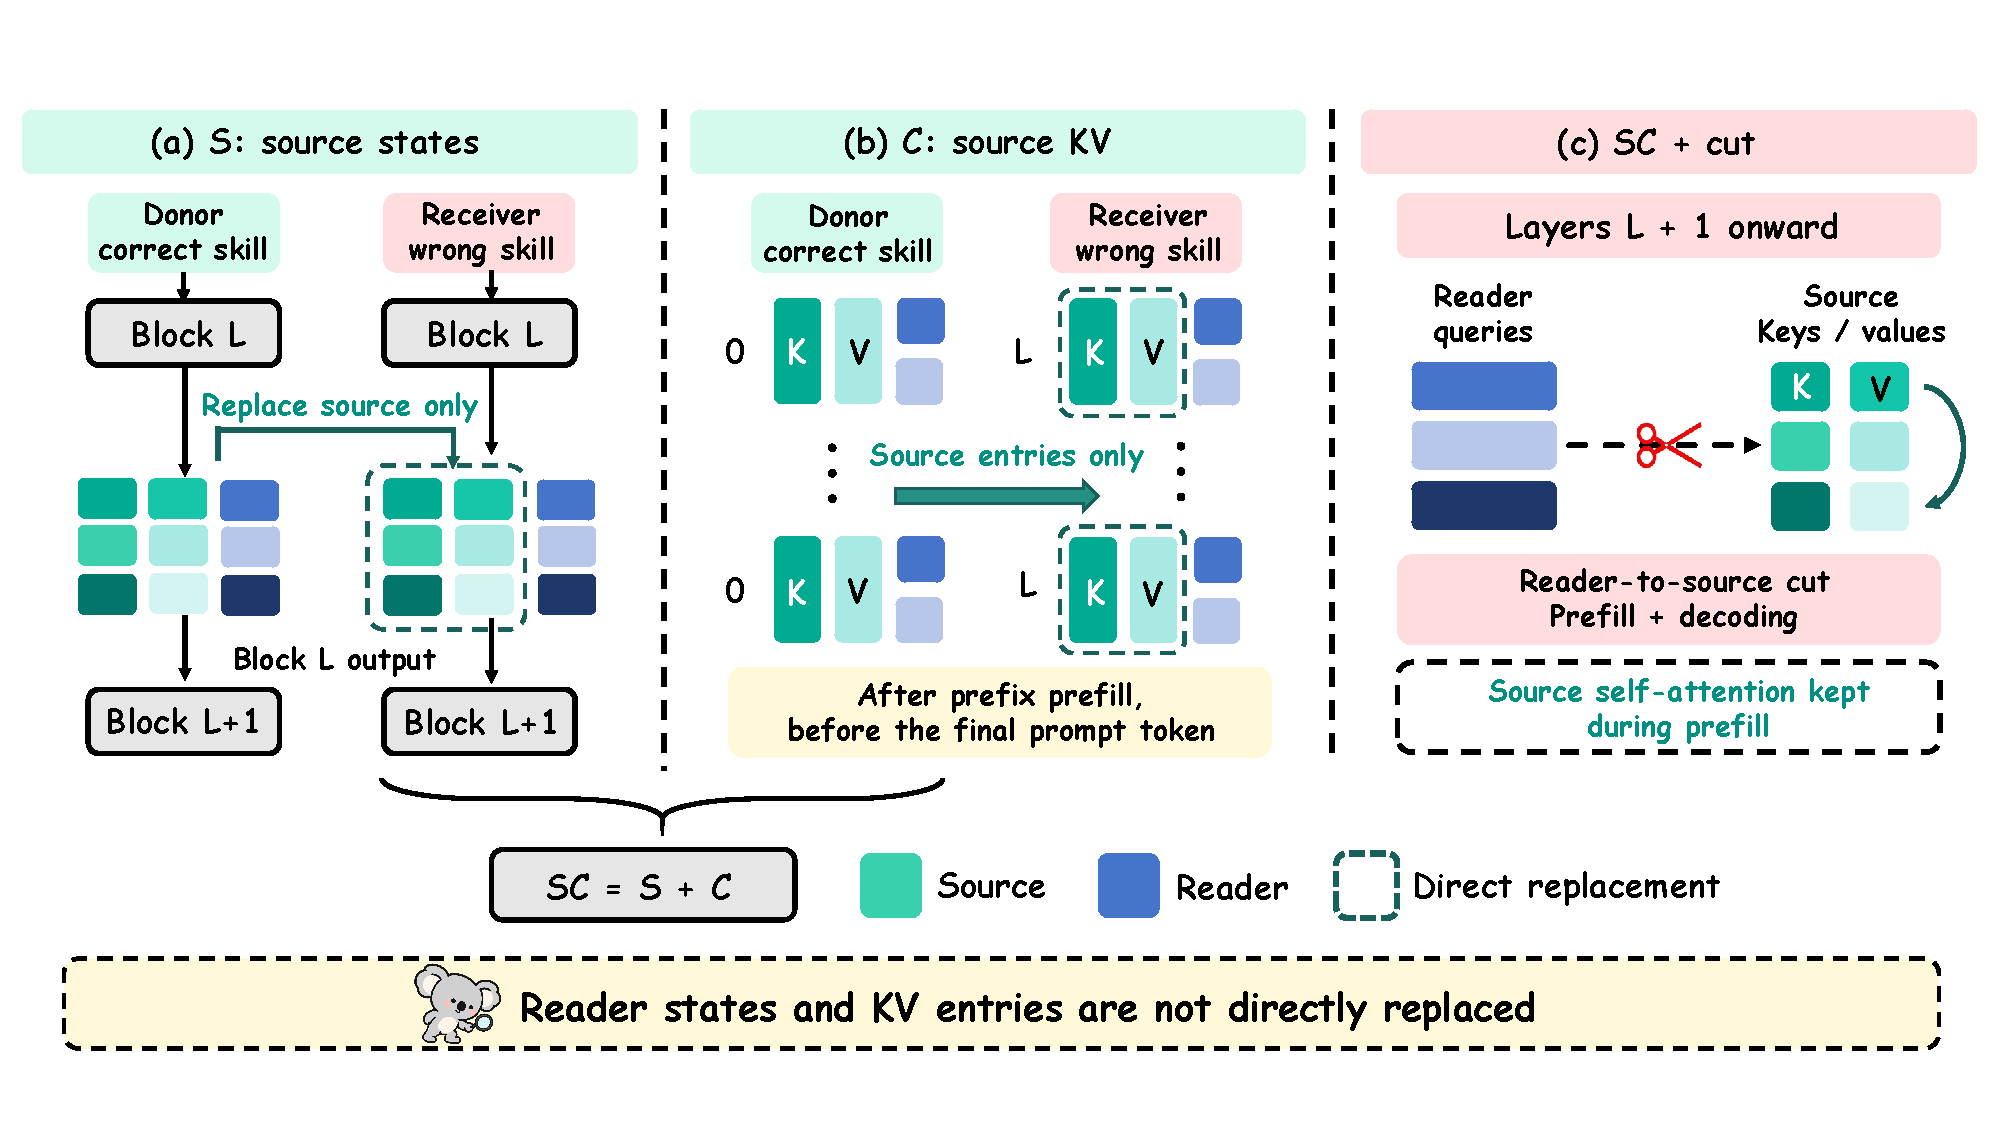
\includegraphics[width=\textwidth]{fig-intervention-design.pdf}
\caption{Timing of state repair, cache repair and the reading cut in the receiver.
The prefix contains all prompt tokens except the last.
(a) $S$ copies donor source states at block $L$'s output during prefix prefill.
(b) $C$ copies source-position key/value (KV) entries at layers $0$ through
$L$ after prefix prefill, before final-token recomputation. $SC$ combines
these two writes, then recomputes the final prompt token and generates.
(c) $SC+\mathrm{cut}$ installs a reading mask before prefill, blocking
reader-to-source attention from $L+1$ onward during prefill and decoding.
Source-to-source attention remains unmasked. Reader states and caches
evolve through computation rather than direct replacement.
Figure~\ref{fig:mechanism}(b) separately tests cuts in the original correct-skill run.}
\Description{Three panels illustrate source-state replacement at block L's
output, source-key/value replacement at layers zero through L, and joint
replacement with a reader-to-source attention cut from layer L plus one.
Green cells mark source positions, blue cells mark readers, and dashed teal
outlines mark direct replacements. The cut applies during prefill and
decoding while source self-attention remains unmasked during prefill.}
\label{fig:design}
\end{figure*}

\paragraph{Hidden-state transfer.}
Each Transformer block is a processing layer that updates the token
vectors. Let $H^L$ denote its output at layer $L$, also called residual
states. Subscripts $D$ and $R$ denote donor and receiver.
State replacement, labelled $S$, writes
\begin{equation}
S:\qquad H_R^L[\mathcal I]\leftarrow H_D^L[\mathcal I].
\label{eq:inject}
\end{equation}
The write occurs during prefill, after which the receiver continues with
the patched states. Other positions at that layer remain unchanged.

\paragraph{Blocking attention to the skill.}
In the original correct-skill execution, we block attention to source
positions at a chosen layer $L$ and every subsequent layer. We call this
\emph{cumulative source-attention knockout}. In attention, a query vector
scores keys at available positions, and the resulting weights combine
their value vectors. Let $z^\ell_{ij}$ be the
attention score from query position $i$ to key position $j$, including the
causal mask that blocks future tokens. At each layer $\ell\ge L$, we set
\begin{equation}
\widetilde z^\ell_{ij}=
\begin{cases}
-\infty,&j\in\mathcal I,\\
z^\ell_{ij},&j\notin\mathcal I.
\end{cases}
\label{eq:knockout}
\end{equation}
The softmax operation converts scores into weights that sum to one.
It gives blocked positions zero weight and normalizes the remaining
weights. An attention head is one of the block's parallel attention
components. The cut applies to all query positions and attention heads during
prefill and decoding. It blocks both readers' access to the skill and
attention within the skill itself, so its effect measures aggregate
source-attention dependence.

The repair extension adds source-cache replacement, denoted $C$, and
combines it with state replacement as $SC$. Figure~\ref{fig:design}
previews these operations, whose layer coverage is defined below.



\paragraph{Recovery and dependence.}
Write $a_D$, $a_R$ and $a_I$ for answer accuracy under the donor, receiver
and an intervention $I$. Recovery is the fraction of the donor's gain
restored in the receiver:
\begin{equation}
\rho(I)=\frac{a_I-a_R}{a_D-a_R}.
\label{eq:rho}
\end{equation}
We require $a_D>a_R$. Thus $\rho=1$ restores that gain and $\rho>1$ exceeds donor accuracy.
For state replacement at layer $L$, we write $\rho(L)$. All three
accuracies use the same items and the transfer protocol's own unpatched
baselines. Section~\ref{sec:setup} defines the evaluation sets.

For knockout, let $q(L)$ be the fraction of eligible, originally correct
answers that remain correct. Source-attention dependence is
\begin{equation}
d(L)=1-q(L).
\label{eq:dependence}
\end{equation}
Higher $d$ means more correct answers are lost when source attention is
blocked. We compare $\rho$ and $d$ on common eligible question IDs, while
retaining each test's baselines. The two measures describe restoration in
the receiver and dependence in the donor. A separate paired-outcome check tests
whether individual questions fail both interventions.

\paragraph{Depth boundaries.}
After establishing effective early transfer, we summarize the curves by
their first half-effect boundaries:
\begin{equation}
\begin{aligned}
T&=\min\{L:\rho(L)<0.5\},\\
R&=\min\{L:d(L)\le0.5\},\qquad \Delta=R-T.
\end{aligned}
\label{eq:boundaries}
\end{equation}
We report these boundaries when both crossings exist.
The separation set $\mathcal W=\{L:\rho(L)<0.5,\ d(L)>0.5\}$ contains
layers with weak transfer and strong source dependence. This set may
contain several intervals. The thresholds summarize half-effect sizes,
and Figure~\ref{fig:transferreading} retains later threshold crossings.
Depth indexes processing layers within each token's computation.

\paragraph{The execution state before generation.}
For one question, split the complete $n$-token prompt before its last token
$u_*$. The processed prefix has positions $\mathcal P=\{0,\ldots,n-2\}$,
including the skill and question. Let
$\overline{\mathcal I}=\mathcal P\setminus\mathcal I$.
Attention reuses cached keys and values for these processed tokens
\citep{shazeer2019fast}. At this point, define
$\mathcal C_X^\ell[\mathcal I]=(K_X^\ell[\mathcal I],V_X^\ell[\mathcal I])$,
collect all layers as $\mathcal C_X[\mathcal I]$, and write
$\mathcal B_X=\mathcal C_X[\overline{\mathcal I}]$ for the other prefix
caches. With model parameters $\theta$, positions, stopping rule and
greedy decoding fixed, the continuation is
\begin{equation}
\hat y_X=\mathcal G_{\theta,M_X}
       (u_*,\mathcal C_X[\mathcal I],\mathcal B_X).
\label{eq:continuation}
\end{equation}
Here $M_X$ specifies attention masks, and $\mathcal G$ includes computing
$u_*$ and generating the answer from both source and other prefix caches.

\paragraph{Cache replacement and joint repair.}
After prefix prefill and before computing $u_*$, cache replacement writes
\begin{equation}
C:\quad \mathcal C_X^\ell[\mathcal I]
 \leftarrow\mathcal C_D^\ell[\mathcal I],\qquad 0\le\ell\le L.
\label{eq:cache}
\end{equation}
The prefix is computed without state replacement for $C$ ($X=R$), or
with the block-$L$ write for $SC$ ($X=S$). The post-prefill write preserves
the other prefix caches. Thus $\mathcal B_C=\mathcal B_R$ and
$\mathcal B_{SC}=\mathcal B_S$, although $\mathcal B_S$ can differ from
$\mathcal B_R$ through indirect effects of $S$.
Under the causal assumptions in Appendix~\ref{app:cache-coverage}, ideal
state replacement reconstructs source KV at layers above $L$. The explicit
cache write supplies layers $0$ through $L$, giving donor-aligned source
caches under $SC$ while retaining the receiver's other prefix caches
$\mathcal B_S$. Figure~\ref{fig:design} shows the write schedule.

\paragraph{From cache repair to output recovery.}
At this same observation point, flatten the prefix caches into
$\mathbf z_X=(\mathbf c_X,\mathbf b_X)$, where $\mathbf c_X$ contains
exactly the source KV entries at layers $0,\ldots,L$.
The remaining vector $\mathbf b_X$ includes higher-layer source KV as well as
$\mathcal B_X$. Adding the cache write to $S$ gives
$\mathbf z_{SC}=(\mathbf c_D,\mathbf b_S)$ without changing
$\mathbf b_S$. For $\varepsilon_X=\|\mathbf z_X-\mathbf z_D\|_2$,
\begin{equation}
\begin{aligned}
\varepsilon_S^2
 &=\|\mathbf c_S-\mathbf c_D\|_2^2+\|\mathbf b_S-\mathbf b_D\|_2^2,\\
\varepsilon_{SC}^2&=\|\mathbf b_S-\mathbf b_D\|_2^2,\\
\varepsilon_S^2-\varepsilon_{SC}^2
 &=\|\mathbf c_S-\mathbf c_D\|_2^2\ge0.
\end{aligned}
\label{eq:cache-distance}
\end{equation}
Here $\|\cdot\|_2$ is the Euclidean length of a vector.
For an exact copy, the coordinate decomposition proves that the squared
cache distance decreases by precisely the replaced entries' squared error,
independently of the causal reconstruction claim above.
Appendix~\ref{app:behavior-recovery} gives a sufficient condition for
donor decoding: at every step, the change in each unnormalized token score,
called a logit, must be less than half the donor's margin. The margin is
the difference between its highest and second-highest scores.
The condition includes cache updates and stopping.

\begin{samepage}
\paragraph{Reading cuts and their timing.}
A \emph{skill-reading cut} blocks reader-to-source attention.
A \emph{within-skill attention cut} blocks source-to-source attention.
In $SC+\mathrm{cut}$, the reading mask is
\begin{equation}
\widetilde z^\ell_{ij}=
\begin{cases}
-\infty,&\ell\ge L+1,\ i\in\mathcal J,\ j\in\mathcal I,\\
z^\ell_{ij},&\text{otherwise}.
\end{cases}
\label{eq:reading-cut}
\end{equation}
\end{samepage}
It is installed before prefix prefill and persists during decoding.
Source-to-source attention remains unmasked, but reader computation can
change already during prefill. Consequently both $M_X$ and
$\mathcal B_X$ in Eq.~\eqref{eq:continuation} can differ from $SC$.
The separate original-run path tests start their cuts at $L$, not $L+1$.
Adding a within-skill cut to a persistent reading cut is structurally
redundant for the output (Appendix~\ref{app:mechanism}).

\paragraph{Three repair contrasts.}
On one fixed evaluation set under one protocol, let $a_X(L)$ denote
accuracy for condition $X$. Suppressing $L$ on the right, define
\begin{equation}
\begin{aligned}
\Delta_{\mathrm{cache}}(L)&=a_{SC}-a_S,\\
\Gamma(L)&=(a_{SC}-a_S)-(a_C-a_R),\\
\Delta_{\mathrm{read}}(L)&=a_{SC}-a_{SC+\mathrm{cut}}.
\end{aligned}
\label{eq:repair-effects}
\end{equation}
These measure the added cache benefit, the interaction on the accuracy
scale, and sensitivity of joint repair to a reading cut.
Positive $\Gamma$ means the joint gain exceeds the sum of the individual
gains. These are intervention contrasts on the accuracy scale.
Multiplying them by $100$ gives percentage points.
